
%Team 17 PRML 
%%%%%%%%%%%%%%%%%%%%%%%%%%%%%%%%%%%%%%%%%%%%%%%%%%%%%%%%%%%%%%%%%%%%%%

%%%%%%%%%%%%%%%%%%%%%%%%%%%%%%%%%%%%%%%%%%%%%%%%%%%%%%%%%%%%%%%%%%%%%%
%
% --------------------------------------------------------------------
% Preamble
% --------------------------------------------------------------------
\documentclass[ fontsize=12pt,twoside]{scrartcl}	

%\setmainfont{Times New Roman}
\usepackage[letterpaper,pdftex]{geometry}	
\setlength{\oddsidemargin}{5mm}			
\setlength{\evensidemargin}{5mm}

\usepackage[table]{xcolor}

\usepackage[english]{babel}
\usepackage[protrusion=true,expansion=true]{microtype}	
\usepackage{amsmath,amsfonts,amsthm,amssymb}
\usepackage{graphicx}
\usepackage{pseudocode}

%\usepackage{titlesec}
%\titlespacing*{\section}{0ex}{0ex}

\setlength{\parindent}{0pt}
\setlength{\parskip}{0.75em}

\usepackage[latin1]{inputenc}
\usepackage{tikz}
\usepackage{subcaption}
\captionsetup{compatibility=false}
%\usepackage[table]{xcolor}
\usetikzlibrary{shapes,arrows}

%Defining the table environment
\setlength{\arrayrulewidth}{0.5mm}
\setlength{\tabcolsep}{20pt}
\renewcommand{\arraystretch}{1.25}



\usepackage{hyperref}
\hypersetup{
    colorlinks=true,
    linkcolor=blue,
    filecolor=magenta,      
    urlcolor=green,
}

% Defining the sections to have roman numerals
\renewcommand{\thesection}{\Roman{section}} 
%\renewcommand{\thesubsection}{\thesection.\Roman{subsection}}
% --------------------------------------------------------------------
% Definitions (do not change this)
% --------------------------------------------------------------------
\newcommand{\HRule}[1]{\rule{\linewidth}{#1}} 	% Horizontal rule

\makeatletter							% Title
\def\printtitle{%						
    {\centering \@title\par}}
\makeatother									

\makeatletter							% Author
\def\printauthor{%					
    {\centering \Large \@author}}				
\makeatother							

% --------------------------------------------------------------------
% Metadata (Change this)
% --------------------------------------------------------------------
\title{	\Large \textsc{ CS5691: Pattern Recognition and Machine Learning \\ 
														Programming	Assignment II} 	
		 	\\[2.0cm]								
			\HRule{2pt} \\						
			\LARGE \textbf{\uppercase{Pattern Classification}}	% Title
			\HRule{2pt} \\ [0.5cm]	
			\Large \today			
		}

 \author{
		Aanand Krishnan {\textit{\small(BE17B001)}}\\	
		Manoranjan J \textit{\small (NA17B112)}\\	
        Reneeth Krishna MG \textit{\small (BS17B025)} \\
        \texttt{Team 17 - CCS Section Spring 2021} \\
}







\begin{document}
% ------------------------------------------------------------------------------
% Maketitle
% ------------------------------------------------------------------------------
\thispagestyle{empty}		

\printtitle					
  	\vfill
\printauthor				
\newpage
% ------------------------------------------------------------------------------
% Begin document
% ------------------------------------------------------------------------------
\setcounter{page}{1}		


%%%%%%%%%%%%%%%
%														%
% 			Main Contents            %
%														%
%%%%%%%%%%%%%%%
\tableofcontents
\listoftables
\listoffigures

\newpage
\section*{}
\section*{Classification}
  In the previous assignment we performed regression, in which the target variable was simply a real valued vector. However, in classification the task is of organizing data into categories for it's efficient use. A shorthand way of saying this would be, the output variable in regression takes continuous values, whereas in classification the output variables takes class labels. For the classification problem at hand, the input feature vector to the model takes numerical attributes. The task of the model then is to assign a class label for the given feature vector.
 
 To build an intuition for the process of classification one could think of a numerical input that has only two features. \textit{For example}, height and weight of several individuals as input for classification as adult and child. Now the classification task is to assign a class (child or adult) to a new unlabelled observation. Such an 2D features input can be easily visualized and the class of a new observation can be inferred from the plots by a very reasonable assumption that the class of the unlabelled point is determined predominantly by nearby points of the training dataset. An interesting observation to note is that, there  was  no  intrinsic  geometry  or  vectors in the example of classification mentioned above or for any classification task for that matter, but by viewing them as vectors we get a geometric intuition that is extremely helpful.
 
 However a severe pitfall of this approach is outlined in chapter one of Bishop. The author points out how with an increase in the number of features, the nearby distance we would scan to make an classification also increases drastically. Such an increase in distance demands an equally drastic increase in number of training data available, making the process infeasible for more than a few featured input. This difficulties arising in higher dimensions is referred to as \textit{curse of dimensionality} in literature. 
 
 This curse however doesn't impair our ability to build machine learning models for real world data that has several thousands features. Bishop, points out a reason for this is that we could essentially capture the variance shown by the data with a subset of features projected on to a different space which has lower dimensions, thus confining the data. Now that we are aware of the effect of dimension, a brief account of how we could model a classification task is provided below. 
 
 \subsection*{Bayesian Decision Theory}
 
 One could abstract the entirety of the models used in machine learning as being developed from minimising different kind of loss functions. In function approximation we minimised the squared distance loss function to make predictions. Bayesian Decision Theory for classification task, is based on a probabilistic loss function. In other words the problem is posed in Probabilistic terms.  \par
 A supervised classification task involves labelled training data,
 \[D = \{(x_1,y_1),(x_2,y_2),\dots, (x_n,y_n)\}\]. The training data is used for learning, following which one of the following methods is followed for prediction,
 
 \begin{itemize}
     \item Using Bayes Theorem,
                   \[  p(Y = y_i|\bar{x}) = \frac{p(\bar{x}|y_i).p(y_i)}{p(x)}  \]
            Now we estimate the posterior class probabilities $p(x|y)$. We can use the joint distribution $p(x,y)$. This kind of methods in which attention is paid to probability distributions of both $x$ and $y$ are known as \textit{generative models}.
     \item In the previous case we were given an $x$, which needed classification. What if we could find a function $f$, that could map each inputs of $x$ to a class label? Such a function, $f$ is called \textit{discriminant}. This kind of models are shown to computationally efficient than the former. A discriminant function can be any one of the following,
     \[
         g_i(\bar{x}) = \begin{cases}  
         
                   p(Y=y_i|\bar{x}), \\
                   
                  p(\bar{x}|Y=y_i).p(Y=y_i), \\
                  
                  \ln{p(\bar{x}|Y=y_i)} + \ln{p(Y=y_i)}
                  
         \end{cases}
     \]
     
     Where the class label $i$ is chosen for which $g_i(\bar{x})$ is maximum. The discriminant function can also be used to find the decision region for a class. $g_i(\bar{x}) - g_j(\bar{x}) = 0 $, gives the decision surface seperating the two classes $i$ and $j$.
     
 
 \end{itemize}
 
 
 \subsubsection*{Gaussian Mixture Model}
 
 This is a discriminant model. In determining the discriminant function several assumptions need to be made, one major assumption of this model is that,
 \[
 p(\bar{x}|y_i) = \sum_{q=1}^{Q} w_q \mathcal{N}(\bar{x}|\bar{\mu}_{iq},\bar{c}_{iq})
 \]
 That is, the class likelihood function is assumed to be a multimodal multivariate Gaussian distribution with $Q-$ peaks. Such an distribution better suits the real world data, for that too contains multiple peaks opposed to the unimodal Gaussian which has a single peak. $w_q$ is scaling factor to adjust for the peak of the distribution with the peak observed in data. 
 
 \[\text{Number of parameters for class i} = Q_i\left(1 + d + \frac{d(d+1)}{2}\right)\]
 
  We could further make assumptions to reduce the number of parameters such that the covariance matrices are equal or covariance matrices are diagonal (\textit{naive} Bayes classifier) and such. Posterior probability for a point to belong a Gaussian component of a particular class is denoted by $\gamma_{nq}$ and is also called the responsibility term. An expression for the responsibility term is,
 
 \[ \gamma_{nq} = \frac{w_q\mathcal{N}(\bar{x}|\bar{\mu}_{q},\bar{c}_{q})}{\sum_{m=1}^{Q}w_m\mathcal{N}(\bar{x}|\bar{\mu}_{m},c_{m})} \]
 
 Maximising this responsibility term using gradient descent we will be able to find out the various parameters of this model. An another advantage of GMM is there might be cases where two classes that are not linearly seperable have the same covariance matrix resulting in a linear decision boundary while using a single Gaussian thus resulting in a poor classification. However there is a hiccup in the parameter estimations for GMM, as it turns out the parameters of this model don't have closed form expression and hence an iterative method known as Expectation-Maximisation(EM) is used.
 
 \newpage
 \subsubsection*{Steps involved in EM method}
 
 \begin{itemize}
     \item [\textbf{Initialization}]
     \item Instead of choosing random values, we divide the data into disjoint sets(clusters) using suitable algorithms such as K-Means. The number of clusters $K$ will be the the hyperparameter $Q$. The rest of the parameters can be estimated as follows,
          \begin{align*}
              N_q &= \text{No. of examples in the $q^{th}$ cluster}\\
              w_q &= \frac{N_q}{N} \\
              \gamma_{nq} &= \begin{cases}  
                               $1$, &\text{if $\bar{x}_n$ \in $q^{th}$ cluster}, \\
                               $0$, &\text{otherwise}
                             \end{cases}\\
              \bar{\mu}_{q} &= \frac{1}{N_q}\sum_{n=1}^{N}\gamma_{nq}.\bar{x}_n \\
              c_q &= \frac{1}{N_q}\sum_{n=1}^{N}\gamma_{nq}(\bar{x}_n -  \bar{\mu}_{q}).(\bar{x}_n -  \bar{\mu}_{q})^t
          \end{align*}
      \item The set of initial parameters $\bar{\theta}^{old}$ is passed on to the next step.
             \[ \bar{\theta}^{old} = \left\{w_q, \bar{\mu}_{q}, c_q    \right\}_{q=1}^{Q}\]
             
      \item [\textbf{Expectation}]
      \item Update the responsibility term as follows,
             \[\gamma_{nq} = \frac{w_q\mathcal{N}(\bar{x}_{n}|\bar{\mu}_{q},c_{q})}{\sum_{m=1}^{Q}w_m\mathcal{N}(\bar{x}_{n}|\bar{\mu}_{m},\c_{m})}\] 
    
      \item [\textbf{Maximization}]
      \item Using the responsibility term obtained in the expectation step, we can estimate $N_q$ which can further be used in the expressions for the other parameters thus updating them all. 
            \[N_q = \sum_{n=1}^{N} \gamma_{nq}\]
      \item The new set of parameters are send on to the next step. The convergence can't be looked at because of the large number of parameters involved. Instead we use a threshold for the stopping criterion as explained in the next step.
           \[ \bar{\theta}^{new} = \left\{w_q^{new}, \bar{\mu}_{q}^{new}, c_q^{new}    \right\}_{q=1}^{Q}\]
      
      \item[\textbf{Likelihood}]  
      \item We estimate the log likelihood as follows,
            \begin{align*}
                \mathcal{L}(D)  &= \sum_{n=1}^{N} \ln{p(\bar{x}_n | \bar{\theta})} \\
                                &= \sum_{n=1}^{N} \ln{\sum_{q=1}^{Q}\mathcal{N}(\bar{x}_n|\bar{\mu}_{q}^{new},c_{q}^{new})}
            \end{align*}
     \item We will look at the increase in likelihood for each updated set of parameters and stop when the difference is below a certain threshold. Else the previous steps are repeated. A guarantee of the EM method is that the the change in the log likelihood will always be positive.
 \end{itemize}
 
 \textbf{Note:} The parameters estimated using EM method are not unique, as what we obtain is a local maximum of the likelihood and not necessarily a global maximum. Hence, the value of the parameters estimated using this method depends on our initialization. Different values of $\bar{\theta}^{old}$  gives different estimates.
 
 
 \subsubsection*{Naive Bayes Classifier}
  This is a special case of the discriminative methods described above. In this model, the density function assumed is a multivariate gaussian function. There is one more important assumption which states that the features are conditionally stastically independent which means that the covariance matrix of the gaussian function is always diagonal which results in lesser parameters to estimate. This function may work well for unimodal data and data in which the features are independent. If the features $x_k$ of the input vector, $\bar{x} = (x_1,x_2,\dots,x_d)$ are independant then,
  
  \begin{align*}
      p(\bar{x}|y_i) &= p(x_1,x_2,\dots,x_d | y_i) \\
                    &= \prod_{k=1}^{d} p(x_k|y_i) \\
                    &= \prod_{k=1}^{d} \mathcal{N}(x_k|\mu_{ik},c_{ik})
  \end{align*}
  
 Mean and covariance are the parameters to be estimated for each class. Since the number of parameters may become high if we consider unique covariance matrices, we sometimes assume the covariance matrix to be same for all classes and in some cases we even assume the diagonal terms are same for the covariance matrices involved to reduce the number of parameters to estimate. These assumptions has its own limitations during the prediction though.

 \subsubsection*{K Nearest Neighbours for density Estimation}
 In this method we assume a different density function than the GMM/naive bayes models we looked at in the previous section. 
 
 \[
 p(\bar{x}|y_i) = \frac{K}{N.V}
 \]
 
 Here \textit{K} is the nearest neighbours to the point in consideration($\bar{x}$) and is fixed for a particular model. \textit{N} is the total number of examples for the class. \textit{V} is the volume that is to be determined which encloses all the K neighbours. Given a particular class and the value K, the only varying entity is the volume \textit{V} for different data points and this plays a role in determining the class for that particular point. This model comes under the non-parametric methods for density estimation which means that there is no weights which has to be optimised for the given data and the prediction of class is based on linear algebra and probability. Thus the class label of $\bar{x}$ upon simplification of the bayes rule is determined by:
 
  \[
 p(y|\bar{x}) = argmin(V_i)
 \]
 
 \subsubsection*{KNN classifier}
 
 This model also comes under non-parametric method for density estimation. We will be assuming the same expression for $p(\bar{x}|y_i)$. But now we try to identify K nearest neighbours for a particular point in consideration based on all the examples and check the number of the neighbour points to different classes and assign the class which has the largest neighbours out of the K points. Thus the class label of $\bar{x}$ upon simplification of the bayes rule is determined by:
 
   \[
 p(y|\bar{x}) = argmax(K_i)
 \]

%------------------------------------------------------

\section{Pattern classification on linearly separable data}
\subsection{\textcolor{teal}{Python Code}}

\begin{minted}[frame=lines, linenos, fontsize=\large]
{python}

#1A part I perceptron

import pandas as pd
import numpy as np
from matplotlib import pyplot as plt
import matplotlib.cm as cm
import matplotlib.colors as colors
from tqdm import tqdm

class perceptron():
    def __init__(self,data1,data2):
        self.data1 = data1
        self.data2 = data2
        self.data = np.concatenate((data1,data2),axis=0)
        self.labels = [data1[0,-1],data2[0,-1]]
        self.weights = None
        self.error_epoch = None
    def train(self,eta,epochs):
        y1 = np.ones((len(self.data1),1))
        y2 = -1*np.ones((len(self.data2),1))
        data = self.data
        N,dim = data[:,:-1].shape
        X = np.concatenate((np.ones((N,1)),data[:,:-1]),axis=1)
        y = np.concatenate((y1,y2),axis=0)
        Xy = np.concatenate((X,np.reshape(y,(len(y),1))),axis=1)
        w = np.random.rand(1,1+dim)
        e = 1
        error_epoch = []
        
        pbar = tqdm(total=epochs,position=0,leave=True)
        while e<=epochs:
            e += 1
            pbar.update(1)
            np.random.shuffle(Xy)
            for i in range(N):
                w = w + ((eta/2)*(Xy[i,-1]-np.sign(Xy[i,:-1]@w.T))*Xy[i,:-1])
            error = 0
            for i in range(N):
                error += (1/2)*abs((Xy[i,-1]-np.sign(Xy[i,:-1]@w.T)))*
                (Xy[i,:-1]@w.T)*Xy[i,-1]
            error_epoch.append(-error)
        pbar.close()
        self.weights = w
        self.error_epoch = np.array(error_epoch)
        return None
    def classify(self,data):
        w = self.weights
        labels = self.labels
        l = [0]+labels 
        return np.array([l[int(i)] for i in np.sign(np.concatenate((np.ones(
        (len(data),1)),data),axis=1)@w.T)])
    def plot_error(self):
        plt.plot(self.error_epoch)
        return None

f = pd.read_csv('17/train.csv',header = None)
data_tr0 = (f[f[2]==0]).to_numpy()
data_tr1 = (f[f[2]==1]).to_numpy()
data_tr2 = (f[f[2]==2]).to_numpy()
data_tr3 = (f[f[2]==3]).to_numpy()
f = pd.read_csv('17/dev.csv',header = None)
data_te0 = (f[f[2]==0]).to_numpy()
data_te1 = (f[f[2]==1]).to_numpy()
data_te2 = (f[f[2]==2]).to_numpy()
data_te3 = (f[f[2]==3]).to_numpy()   

eta = 0.1
epochs = 10
#01
p01 = perceptron(data_tr0,data_tr1)
p01.train(eta,epochs)
data_tr01 = np.concatenate((data_tr0,data_tr1),axis=0)
train_acc_01 = 100*((data_tr01[:,-1]==p01.classify(data_tr01[:,:-1]))
                    .mean())
print('train_acc_01 = %f'%(train_acc_01))
data_te01 = np.concatenate((data_te0,data_te1),axis=0)
test_acc_01 = 100*((data_te01[:,-1]==p01.classify(data_te01[:,:-1]))
                  .mean())
print('test_acc_01 = %f'%(test_acc_01))

#02
p02 = perceptron(data_tr0,data_tr2)
p02.train(eta,epochs)
data_tr02 = np.concatenate((data_tr0,data_tr2),axis=0)
train_acc_02 = 100*((data_tr02[:,-1]==p02.classify(data_tr02[:,:-1]))
                    .mean())
print('train_acc_02 = %f'%(train_acc_02))
data_te02 = np.concatenate((data_te0,data_te2),axis=0)
test_acc_02 = 100*((data_te02[:,-1]==p02.classify(data_te02[:,:-1]))
                .mean())
print('test_acc_02 = %f'%(test_acc_02))

#03
p03 = perceptron(data_tr0,data_tr3)
p03.train(eta,epochs)
data_tr03 = np.concatenate((data_tr0,data_tr3),axis=0)
train_acc_03 = 100*((data_tr03[:,-1]==p03.classify(data_tr03[:,:-1]))
                   .mean())
print('train_acc_03 = %f'%(train_acc_03))
data_te03 = np.concatenate((data_te0,data_te3),axis=0)
test_acc_03 = 100*((data_te03[:,-1]==p03.classify(data_te03[:,:-1]))
                  .mean())
print('test_acc_03 = %f'%(test_acc_03))
#12
p12 = perceptron(data_tr1,data_tr2)
p12.train(eta,epochs)
data_tr12 = np.concatenate((data_tr1,data_tr2),axis=0)
train_acc_12 = 100*((data_tr12[:,-1]==p12.classify(data_tr12[:,:-1]))
                    .mean())
print('train_acc_12 = %f'%(train_acc_12))
data_te12 = np.concatenate((data_te1,data_te2),axis=0)
test_acc_12 = 100*((data_te12[:,-1]==p12.classify(data_te12[:,:-1]))
                  .mean())
print('test_acc_12 = %f'%(test_acc_12))
#13
p13 = perceptron(data_tr1,data_tr3)
p13.train(eta,epochs)
data_tr13 = np.concatenate((data_tr1,data_tr3),axis=0)
train_acc_13 = 100*((data_tr13[:,-1]==p13.classify(data_tr13[:,:-1]))
                   .mean())
print('train_acc_13 = %f'%(train_acc_13))
data_te13 = np.concatenate((data_te1,data_te3),axis=0)
test_acc_13 = 100*((data_te13[:,-1]==p13.classify(data_te13[:,:-1]))
                   .mean())
print('test_acc_13 = %f'%(test_acc_13))
#23
p23 = perceptron(data_tr2,data_tr3)
p23.train(eta,epochs)
data_tr23 = np.concatenate((data_tr2,data_tr3),axis=0)
train_acc_23 = 100*((data_tr23[:,-1]==p23.classify(data_tr23[:,:-1]))
                   .mean())
print('train_acc_23 = %f'%(train_acc_23))
data_te23 = np.concatenate((data_te2,data_te3),axis=0)
test_acc_23 = 100*((data_te23[:,-1]==p23.classify(data_te23[:,:-1]))
                  .mean())
print('test_acc_23 = %f'%(test_acc_23))

#plots
X_train = data_tr01
X_test = data_te01
# Decision Region Plots #####################################################
# define bounds of the domain
min1, max1 = X_train[:, 0].min()-1, X_train[:, 0].max()+1
min2, max2 = X_train[:, 1].min()-1, X_train[:, 1].max()+1

# define the x and y scale
x1_grid = np.arange(min1, max1, 0.1)
x2_grid = np.arange(min2, max2, 0.1)

x1_grid, x2_grid = np.meshgrid(x1_grid, x2_grid)

c1, c2 = x1_grid.flatten(), x1_grid.flatten()
c1, c2 = x1_grid.reshape((len(c1), 1)), x2_grid.reshape((len(c2), 1))

x = np.hstack((c1,c2))

y_pred = p01.classify(x)

x3_grid = y_pred.reshape(x1_grid.shape)



fig = plt.figure(1,figsize=(7.5,4))
ax = fig.add_subplot(111)
cmap =plt.get_cmap('Paired',2)
cs = ax.contourf(x1_grid, x2_grid, x3_grid, cmap=cmap)
ax.scatter(X_train[:,0],X_train[:,1],marker='x',
        color = 'blue',label='train data')
ax.scatter(X_test[:,0],X_test[:,1],marker='x',
        color='black',label='test data')
ax.legend()
ax.set_xlabel('x1',fontsize=10)
ax.set_ylabel('x2',fontsize=10)
ax.set_title('Perceptron : Labels (0,1)', fontsize=10)
cbar = plt.colorbar(cm.ScalarMappable(cmap=cmap),
                    ticks =[0.25,0.75])
cbar.ax.invert_yaxis()
cbar.set_ticklabels(['0','1'])

X_train = data_tr02
X_test = data_te02
# Decision Region Plots #####################################################
# define bounds of the domain
min1, max1 = X_train[:, 0].min()-1, X_train[:, 0].max()+1
min2, max2 = X_train[:, 1].min()-1, X_train[:, 1].max()+1

# define the x and y scale
x1_grid = np.arange(min1, max1, 0.1)
x2_grid = np.arange(min2, max2, 0.1)

x1_grid, x2_grid = np.meshgrid(x1_grid, x2_grid)

c1, c2 = x1_grid.flatten(), x1_grid.flatten()
c1, c2 = x1_grid.reshape((len(c1), 1)),
        x2_grid.reshape((len(c2), 1))

x = np.hstack((c1,c2))

y_pred = p02.classify(x)

x3_grid = y_pred.reshape(x1_grid.shape)



fig = plt.figure(2,figsize=(7.5,4))
ax = fig.add_subplot(111)
cmap =plt.get_cmap('Paired',2)
cs = ax.contourf(x1_grid, x2_grid, x3_grid, cmap=cmap)
ax.scatter(X_train[:,0],X_train[:,1],marker='x',
           color = 'blue',label='train data')
ax.scatter(X_test[:,0],X_test[:,1],marker='x',
             color='black',label='test data')
ax.legend()
ax.set_xlabel('x1',fontsize=10)
ax.set_ylabel('x2',fontsize=10)
ax.set_title('Perceptron : Labels (0,2)', fontsize=10)
cbar = plt.colorbar(cm.ScalarMappable(cmap=cmap),ticks =[0.25,0.75])
cbar.ax.invert_yaxis()
cbar.set_ticklabels(['0','2'])

X_train = data_tr03
X_test = data_te03
# Decision Region Plots #####################################################
# define bounds of the domain
min1, max1 = X_train[:, 0].min()-1, X_train[:, 0].max()+1
min2, max2 = X_train[:, 1].min()-1, X_train[:, 1].max()+1

# define the x and y scale
x1_grid = np.arange(min1, max1, 0.1)
x2_grid = np.arange(min2, max2, 0.1)

x1_grid, x2_grid = np.meshgrid(x1_grid, x2_grid)

c1, c2 = x1_grid.flatten(), x1_grid.flatten()
c1, c2 = x1_grid.reshape((len(c1), 1)),
            x2_grid.reshape((len(c2), 1))

x = np.hstack((c1,c2))

y_pred = p03.classify(x)

x3_grid = y_pred.reshape(x1_grid.shape)



fig = plt.figure(3,figsize=(7.5,4))
ax = fig.add_subplot(111)
cmap =plt.get_cmap('Paired',2)
cs = ax.contourf(x1_grid, x2_grid, x3_grid, cmap=cmap)
ax.scatter(X_train[:,0],X_train[:,1],marker='x',
            color = 'blue',label='train data')
ax.scatter(X_test[:,0],X_test[:,1],marker='x',
           color='black',label='test data')
ax.legend()
ax.set_xlabel('x1',fontsize=10)
ax.set_ylabel('x2',fontsize=10)
ax.set_title('Perceptron : Labels (0,3)', fontsize=10)
cbar = plt.colorbar(cm.ScalarMappable(cmap=cmap),
        ticks =[0.25,0.75])
cbar.ax.invert_yaxis()
cbar.set_ticklabels(['0','3'])

X_train = data_tr12
X_test = data_te12
# Decision Region Plots #####################################################
# define bounds of the domain
min1, max1 = X_train[:, 0].min()-1, X_train[:, 0].max()+1
min2, max2 = X_train[:, 1].min()-1, X_train[:, 1].max()+1

# define the x and y scale
x1_grid = np.arange(min1, max1, 0.1)
x2_grid = np.arange(min2, max2, 0.1)

x1_grid, x2_grid = np.meshgrid(x1_grid, x2_grid)

c1, c2 = x1_grid.flatten(), x1_grid.flatten()
c1, c2 = x1_grid.reshape((len(c1), 1)),
           x2_grid.reshape((len(c2), 1))

x = np.hstack((c1,c2))

y_pred = p12.classify(x)

x3_grid = y_pred.reshape(x1_grid.shape)



fig = plt.figure(4,figsize=(7.5,4))
ax = fig.add_subplot(111)
cmap =plt.get_cmap('Paired',2)
cs = ax.contourf(x1_grid, x2_grid, x3_grid, cmap=cmap)
ax.scatter(X_train[:,0],X_train[:,1],marker='x',
           color = 'blue',label='train data')
ax.scatter(X_test[:,0],X_test[:,1],marker='x',
            color='black',label='test data')
ax.legend()
ax.set_xlabel('x1',fontsize=10)
ax.set_ylabel('x2',fontsize=10)
ax.set_title('Perceptron : Labels (1,2)', fontsize=10)
cbar = plt.colorbar(cm.ScalarMappable(cmap=cmap),
                    ticks =[0.25,0.75])
cbar.ax.invert_yaxis()
cbar.set_ticklabels(['1','2'])

X_train = data_tr13
X_test = data_te13
# Decision Region Plots #####################################################
# define bounds of the domain
min1, max1 = X_train[:, 0].min()-1, X_train[:, 0].max()+1
min2, max2 = X_train[:, 1].min()-1, X_train[:, 1].max()+1

# define the x and y scale
x1_grid = np.arange(min1, max1, 0.1)
x2_grid = np.arange(min2, max2, 0.1)

x1_grid, x2_grid = np.meshgrid(x1_grid, x2_grid)

c1, c2 = x1_grid.flatten(), x1_grid.flatten()
c1, c2 = x1_grid.reshape((len(c1), 1)), 
                    x2_grid.reshape((len(c2), 1))

x = np.hstack((c1,c2))

y_pred = p13.classify(x)

x3_grid = y_pred.reshape(x1_grid.shape)



fig = plt.figure(5,figsize=(7.5,4))
ax = fig.add_subplot(111)
cmap =plt.get_cmap('Paired',2)
cs = ax.contourf(x1_grid, x2_grid, x3_grid, cmap=cmap)
ax.scatter(X_train[:,0],X_train[:,1],marker='x',
            color = 'blue',label='train data')
ax.scatter(X_test[:,0],X_test[:,1],marker='x', 
             color='black',label='test data')
ax.legend()
ax.set_xlabel('x1',fontsize=10)
ax.set_ylabel('x2',fontsize=10)
ax.set_title('Perceptron : Labels (1,3)', fontsize=10)
cbar = plt.colorbar(cm.ScalarMappable(cmap=cmap),
          ticks =[0.25,0.75])
cbar.ax.invert_yaxis()
cbar.set_ticklabels(['1','3'])

X_train = data_tr23
X_test = data_te23
# Decision Region Plots #####################################################
# define bounds of the domain
min1, max1 = X_train[:, 0].min()-1, X_train[:, 0].max()+1
min2, max2 = X_train[:, 1].min()-1, X_train[:, 1].max()+1

# define the x and y scale
x1_grid = np.arange(min1, max1, 0.1)
x2_grid = np.arange(min2, max2, 0.1)

x1_grid, x2_grid = np.meshgrid(x1_grid, x2_grid)

c1, c2 = x1_grid.flatten(), x1_grid.flatten()
c1, c2 = x1_grid.reshape((len(c1), 1)), 
          x2_grid.reshape((len(c2), 1))

x = np.hstack((c1,c2))

y_pred = p23.classify(x)

x3_grid = y_pred.reshape(x1_grid.shape)



fig = plt.figure(6,figsize=(7.5,4))
ax = fig.add_subplot(111)
cmap =plt.get_cmap('Paired',2)
cs = ax.contourf(x1_grid, x2_grid, x3_grid, cmap=cmap)
ax.scatter(X_train[:,0],X_train[:,1],marker='x',
               color = 'blue',label='train data')
ax.scatter(X_test[:,0],X_test[:,1],marker='x',
            color='black',label='test data')
ax.legend()
ax.set_xlabel('x1',fontsize=10)
ax.set_ylabel('x2',fontsize=10)
ax.set_title('Perceptron : Labels (2,3)', fontsize=10)
cbar = plt.colorbar(cm.ScalarMappable(cmap=cmap),
                ticks =[0.25,0.75])
cbar.ax.invert_yaxis()
cbar.set_ticklabels(['2','3'])

#1A part II MLFNN

from sklearn import preprocessing
import pandas as pd
import numpy as np
import torch as tc
from matplotlib import pyplot as plt
import matplotlib.cm as cm
import matplotlib.colors as colors
from tqdm import tqdm

f = pd.read_csv('17/train.csv',header = None)
data_tr = f.to_numpy()
f = pd.read_csv('17/dev.csv',header = None)
data_te = f.to_numpy()
#1 to K categorial 1 hot vector transformation
labelenc = preprocessing.LabelBinarizer()  
Xtr = (tc.from_numpy(data_tr[:,:-1])).float()
ytr = (tc.from_numpy(labelenc.fit_transform(data_tr[:,-1])))
                    .float()
Xte = (tc.from_numpy(data_te[:,:-1])).float()
yte = (tc.from_numpy(labelenc.fit_transform(data_te[:,-1])))
                    .float()

epochs = 10000

inp_l = 2
hid_l = 4
out_l = 4
#activation fxns : Sigmoid,Tanh,SOftmax,ReLU,ELU,SELU,CELU,
mlfnn = tc.nn.Sequential(tc.nn.Linear(inp_l,hid_l),
                         tc.nn.ELU(),tc.nn.Linear(hid_l,out_l))
MSE = tc.nn.MSELoss()
optimizer = tc.optim.SGD(mlfnn.parameters(), lr=0.001)
from tqdm import tqdm
epochs = 10000
pbar = tqdm(total=epochs,position=0,leave=True)
for i in range(epochs):
    
    optimizer.zero_grad() 
    ytrp = mlfnn(Xtr)
    loss = MSE(ytrp,ytr)
    loss.backward()
    optimizer.step()
    pbar.update(1)
pbar.close()
tr_acc = 100*((data_tr[:,-1] == labelenc.
                    inverse_transform(mlfnn(Xtr))).mean())
te_acc = 100*((data_te[:,-1] == labelenc.
                     inverse_transform(mlfnn(Xte))).mean())
print('train acc = %f'%(tr_acc))
print('test acc = %f'%(te_acc))

#plotting
X_train = data_tr[:,:-1]
X_test = data_te[:,:-1]
# Decision Region Plots #####################################################
# define bounds of the domain
min1, max1 = X_train[:, 0].min()-1, X_train[:, 0].max()+1
min2, max2 = X_train[:, 1].min()-1, X_train[:, 1].max()+1

# define the x and y scale
x1_grid = np.arange(min1, max1, 0.1)
x2_grid = np.arange(min2, max2, 0.1)

x1_grid, x2_grid = np.meshgrid(x1_grid, x2_grid)

c1, c2 = x1_grid.flatten(), x1_grid.flatten()
c1, c2 = x1_grid.reshape((len(c1), 1)), x2_grid.
                           reshape((len(c2), 1))

x = np.hstack((c1,c2))

y_pred = labelenc.inverse_transform(mlfnn(tc.from_numpy(x)
                                    .float()))

x3_grid = y_pred.reshape(x1_grid.shape)


fig = plt.figure(1,figsize=(7.5,4))
ax = fig.add_subplot(111)
cmap =plt.get_cmap('Paired',4)
cs = ax.contourf(x1_grid, x2_grid, x3_grid, cmap=cmap)
ax.scatter(X_train[:,0],X_train[:,1],marker='x',
                color = 'blue',label='train data')
ax.scatter(X_test[:,0],X_test[:,1],marker='x',
                  color='black',label='test data')
ax.legend()
ax.set_xlabel('x1',fontsize=10)
ax.set_ylabel('x2',fontsize=10)
ax.set_title('MLFNN : All Four Labels', fontsize=10)
cbar = plt.colorbar(cm.ScalarMappable(cmap=cmap),
                  ticks=np.linspace(0.125,1-0.125,4))
cbar.ax.invert_yaxis()
cbar.set_ticklabels(['0','1','2','3'])

#1A part III linear svm
import numpy as np
import pandas as pd
from sklearn.svm import SVC
from matplotlib import pyplot as plt
import matplotlib.cm as cm
import matplotlib.colors as colors
from tqdm import tqdm

f = pd.read_csv('17/train.csv',header = None)
data_tr0 = (f[f[2]==0]).to_numpy()
data_tr1 = (f[f[2]==1]).to_numpy()
data_tr2 = (f[f[2]==2]).to_numpy()
data_tr3 = (f[f[2]==3]).to_numpy()
f = pd.read_csv('17/dev.csv',header = None)
data_te0 = (f[f[2]==0]).to_numpy()
data_te1 = (f[f[2]==1]).to_numpy()
data_te2 = (f[f[2]==2]).to_numpy()
data_te3 = (f[f[2]==3]).to_numpy()

#01
data_tr01 = np.concatenate((data_tr0,data_tr1),axis=0)
data_te01 = np.concatenate((data_te0,data_te1),axis=0)
svc01 = SVC(kernel='linear')
svc01.fit(data_tr01[:,:-1],data_tr01[:,-1])
train_acc_01 = 100*((data_tr01[:,-1]==svc01.
                    predict(data_tr01[:,:-1])).mean())
print('train_acc_01 = %f'%(train_acc_01))
test_acc_01 = 100*((data_te01[:,-1]==svc01.
                    predict(data_te01[:,:-1])).mean())
print('test_acc_01 = %f'%(test_acc_01))

#02
data_tr02 = np.concatenate((data_tr0,data_tr2),axis=0)
data_te02 = np.concatenate((data_te0,data_te2),axis=0)
svc02 = SVC(kernel='linear')
svc02.fit(data_tr02[:,:-1],data_tr02[:,-1])
train_acc_02 = 100*((data_tr02[:,-1]==svc02.
                    predict(data_tr02[:,:-1])).mean())
print('train_acc_02 = %f'%(train_acc_02))
test_acc_02 = 100*((data_te02[:,-1]==svc02.
                    predict(data_te02[:,:-1])).mean())
print('test_acc_02 = %f'%(test_acc_02))

#03
data_tr03 = np.concatenate((data_tr0,data_tr3),axis=0)
data_te03 = np.concatenate((data_te0,data_te3),axis=0)
svc03 = SVC(kernel='linear')
svc03.fit(data_tr03[:,:-1],data_tr03[:,-1])
train_acc_03 = 100*((data_tr03[:,-1]==svc03.
                    predict(data_tr03[:,:-1])).mean())
print('train_acc_03 = %f'%(train_acc_03))
test_acc_03 = 100*((data_te03[:,-1]==svc03.
                     predict(data_te03[:,:-1])).mean())
print('test_acc_03 = %f'%(test_acc_03))

#12
data_tr12 = np.concatenate((data_tr1,data_tr2),axis=0)
data_te12 = np.concatenate((data_te1,data_te2),axis=0)
svc12 = SVC(kernel='linear')
svc12.fit(data_tr12[:,:-1],data_tr12[:,-1])
train_acc_12 = 100*((data_tr12[:,-1]==svc12.
                      predict(data_tr12[:,:-1])).mean())
print('train_acc_12 = %f'%(train_acc_12))
test_acc_12 = 100*((data_te12[:,-1]==svc12.
                       predict(data_te12[:,:-1])).mean())
print('test_acc_12 = %f'%(test_acc_12))

#13
data_tr13 = np.concatenate((data_tr1,data_tr3),axis=0)
data_te13 = np.concatenate((data_te1,data_te3),axis=0)
svc13 = SVC(kernel='linear')
svc13.fit(data_tr13[:,:-1],data_tr13[:,-1])
train_acc_13 = 100*((data_tr13[:,-1]==svc13.
                       predict(data_tr13[:,:-1])).mean())
print('train_acc_13 = %f'%(train_acc_13))
test_acc_13 = 100*((data_te13[:,-1]==svc13.
                       predict(data_te13[:,:-1])).mean())
print('test_acc_13 = %f'%(test_acc_13))

#23
data_tr23 = np.concatenate((data_tr2,data_tr3),axis=0)
data_te23 = np.concatenate((data_te2,data_te3),axis=0)
svc23 = SVC(kernel='linear')
svc23.fit(data_tr23[:,:-1],data_tr23[:,-1])
train_acc_23 = 100*((data_tr23[:,-1]==svc23.
                      predict(data_tr23[:,:-1])).mean())
print('train_acc_23 = %f'%(train_acc_23))
test_acc_23 = 100*((data_te23[:,-1]==svc23.
                      predict(data_te23[:,:-1])).mean())
print('test_acc_23 = %f'%(test_acc_23))

#plots
X_train = data_tr01
X_test = data_te01
# Decision Region Plots #####################################################
# define bounds of the domain
min1, max1 = X_train[:, 0].min()-1, X_train[:, 0].max()+1
min2, max2 = X_train[:, 1].min()-1, X_train[:, 1].max()+1

# define the x and y scale
x1_grid = np.arange(min1, max1, 0.1)
x2_grid = np.arange(min2, max2, 0.1)

x1_grid, x2_grid = np.meshgrid(x1_grid, x2_grid)

c1, c2 = x1_grid.flatten(), x1_grid.flatten()
c1, c2 = x1_grid.reshape((len(c1), 1)), x2_grid.
                         reshape((len(c2), 1))

x = np.hstack((c1,c2))

y_pred = svc01.predict(x)

x3_grid = y_pred.reshape(x1_grid.shape)

suppvec = svc01.support_vectors_

fig = plt.figure(1,figsize=(7.5,4))
ax = fig.add_subplot(111)
cmap =plt.get_cmap('Paired',2)
cs = ax.contourf(x1_grid, x2_grid, x3_grid, cmap=cmap)
ax.scatter(X_train[:,0],X_train[:,1],marker='x',
                     color = 'blue',label='train data')
ax.scatter(suppvec[:,0],suppvec[:,1],marker='x',
                  color='yellow',label='support vector')
ax.scatter(X_test[:,0],X_test[:,1],marker='x',
                         color='black',label='test data')
ax.legend()
ax.set_xlabel('x1',fontsize=10)
ax.set_ylabel('x2',fontsize=10)
ax.set_title('SVM : Labels (0,1)', fontsize=10)
cbar = plt.colorbar(cm.ScalarMappable(cmap=cmap),
                             ticks =[0.25,0.75])
cbar.ax.invert_yaxis()
cbar.set_ticklabels(['0','1'])



X_train = data_tr02
X_test = data_te02
# Decision Region Plots #####################################################
# define bounds of the domain
min1, max1 = X_train[:, 0].min()-1, X_train[:, 0].max()+1
min2, max2 = X_train[:, 1].min()-1, X_train[:, 1].max()+1

# define the x and y scale
x1_grid = np.arange(min1, max1, 0.1)
x2_grid = np.arange(min2, max2, 0.1)

x1_grid, x2_grid = np.meshgrid(x1_grid, x2_grid)

c1, c2 = x1_grid.flatten(), x1_grid.flatten()
c1, c2 = x1_grid.reshape((len(c1), 1)), 
             x2_grid.reshape((len(c2), 1))

x = np.hstack((c1,c2))

y_pred = svc02.predict(x)

x3_grid = y_pred.reshape(x1_grid.shape)

suppvec = svc02.support_vectors_

fig = plt.figure(2,figsize=(7.5,4))
ax = fig.add_subplot(111)
cmap =plt.get_cmap('Paired',2)
cs = ax.contourf(x1_grid, x2_grid, x3_grid, cmap=cmap)
ax.scatter(X_train[:,0],X_train[:,1],marker='x',
             color = 'blue',label='train data')
ax.scatter(suppvec[:,0],suppvec[:,1],marker='x',
            color='yellow',label='support vector')
ax.scatter(X_test[:,0],X_test[:,1],marker='x',
                  color='black',label='test data')
ax.legend()
ax.set_xlabel('x1',fontsize=10)
ax.set_ylabel('x2',fontsize=10)
ax.set_title('SVM : Labels (0,2)', fontsize=10)
cbar = plt.colorbar(cm.ScalarMappable(cmap=cmap),
                            ticks =[0.25,0.75])
cbar.ax.invert_yaxis()
cbar.set_ticklabels(['0','2'])

X_train = data_tr03
X_test = data_te03
# Decision Region Plots #####################################################
# define bounds of the domain
min1, max1 = X_train[:, 0].min()-1, X_train[:, 0].max()+1
min2, max2 = X_train[:, 1].min()-1, X_train[:, 1].max()+1

# define the x and y scale
x1_grid = np.arange(min1, max1, 0.1)
x2_grid = np.arange(min2, max2, 0.1)

x1_grid, x2_grid = np.meshgrid(x1_grid, x2_grid)

c1, c2 = x1_grid.flatten(), x1_grid.flatten()
c1, c2 = x1_grid.reshape((len(c1), 1)), x2_grid.
                            reshape((len(c2), 1))

x = np.hstack((c1,c2))

y_pred = svc03.predict(x)

x3_grid = y_pred.reshape(x1_grid.shape)

suppvec = svc03.support_vectors_

fig = plt.figure(3,figsize=(7.5,4))
ax = fig.add_subplot(111)
cmap =plt.get_cmap('Paired',2)
cs = ax.contourf(x1_grid, x2_grid, x3_grid, cmap=cmap)
ax.scatter(X_train[:,0],X_train[:,1],marker='x',
                color = 'blue',label='train data')
ax.scatter(suppvec[:,0],suppvec[:,1],marker='x',
            color='yellow',label='support vector')
ax.scatter(X_test[:,0],X_test[:,1],marker='x',
                  color='black',label='test data')
ax.legend()
ax.set_xlabel('x1',fontsize=10)
ax.set_ylabel('x2',fontsize=10)
ax.set_title('SVM : Labels (0,3)', fontsize=10)
cbar = plt.colorbar(cm.ScalarMappable(cmap=cmap),
                             ticks =[0.25,0.75])
cbar.ax.invert_yaxis()
cbar.set_ticklabels(['0','3'])

X_train = data_tr12
X_test = data_te12
# Decision Region Plots #####################################################
# define bounds of the domain
min1, max1 = X_train[:, 0].min()-1, X_train[:, 0].max()+1
min2, max2 = X_train[:, 1].min()-1, X_train[:, 1].max()+1

# define the x and y scale
x1_grid = np.arange(min1, max1, 0.1)
x2_grid = np.arange(min2, max2, 0.1)

x1_grid, x2_grid = np.meshgrid(x1_grid, x2_grid)

c1, c2 = x1_grid.flatten(), x1_grid.flatten()
c1, c2 = x1_grid.reshape((len(c1), 1)), x2_grid.
                           reshape((len(c2), 1))

x = np.hstack((c1,c2))

y_pred = svc12.predict(x)

x3_grid = y_pred.reshape(x1_grid.shape)

suppvec = svc12.support_vectors_

fig = plt.figure(4,figsize=(7.5,4))
ax = fig.add_subplot(111)
cmap =plt.get_cmap('Paired',2)
cs = ax.contourf(x1_grid, x2_grid, x3_grid, cmap=cmap)
ax.scatter(X_train[:,0],X_train[:,1],marker='x',
               color = 'blue',label='train data')
ax.scatter(suppvec[:,0],suppvec[:,1],marker='x',
             color='yellow',label='support vector')
ax.scatter(X_test[:,0],X_test[:,1],marker='x',
                  color='black',label='test data')
ax.legend()
ax.set_xlabel('x1',fontsize=10)
ax.set_ylabel('x2',fontsize=10)
ax.set_title('SVM : Labels (1,2)', fontsize=10)
cbar = plt.colorbar(cm.ScalarMappable(cmap=cmap),
                             ticks =[0.25,0.75])
cbar.ax.invert_yaxis()
cbar.set_ticklabels(['1','2'])

X_train = data_tr13
X_test = data_te13
# Decision Region Plots #####################################################
# define bounds of the domain
min1, max1 = X_train[:, 0].min()-1, X_train[:, 0].max()+1
min2, max2 = X_train[:, 1].min()-1, X_train[:, 1].max()+1

# define the x and y scale
x1_grid = np.arange(min1, max1, 0.1)
x2_grid = np.arange(min2, max2, 0.1)

x1_grid, x2_grid = np.meshgrid(x1_grid, x2_grid)

c1, c2 = x1_grid.flatten(), x1_grid.flatten()
c1, c2 = x1_grid.reshape((len(c1), 1)), x2_grid.
                           reshape((len(c2), 1))

x = np.hstack((c1,c2))

y_pred = svc13.predict(x)

x3_grid = y_pred.reshape(x1_grid.shape)

suppvec = svc13.support_vectors_

fig = plt.figure(5,figsize=(7.5,4))
ax = fig.add_subplot(111)
cmap =plt.get_cmap('Paired',2)
cs = ax.contourf(x1_grid, x2_grid, x3_grid, cmap=cmap)
ax.scatter(X_train[:,0],X_train[:,1],marker='x',
                       color = 'blue',label='train data')
ax.scatter(suppvec[:,0],suppvec[:,1],marker='x',
                   color='yellow',label='support vector')
ax.scatter(X_test[:,0],X_test[:,1],marker='x',
                        color='black',label='test data')
ax.legend()
ax.set_xlabel('x1',fontsize=10)
ax.set_ylabel('x2',fontsize=10)
ax.set_title('SVM : Labels (1,3)', fontsize=10)
cbar = plt.colorbar(cm.ScalarMappable(cmap=cmap),ticks =[0.25,0.75])
cbar.ax.invert_yaxis()
cbar.set_ticklabels(['1','3'])

X_train = data_tr23
X_test = data_te23
# Decision Region Plots #####################################################
# define bounds of the domain
min1, max1 = X_train[:, 0].min()-1, X_train[:, 0].max()+1
min2, max2 = X_train[:, 1].min()-1, X_train[:, 1].max()+1

# define the x and y scale
x1_grid = np.arange(min1, max1, 0.1)
x2_grid = np.arange(min2, max2, 0.1)

x1_grid, x2_grid = np.meshgrid(x1_grid, x2_grid)

c1, c2 = x1_grid.flatten(), x1_grid.flatten()
c1, c2 = x1_grid.reshape((len(c1), 1)), x2_grid.
                           reshape((len(c2), 1))

x = np.hstack((c1,c2))

y_pred = svc23.predict(x)

x3_grid = y_pred.reshape(x1_grid.shape)

suppvec = svc23.support_vectors_

fig = plt.figure(6,figsize=(7.5,4))
ax = fig.add_subplot(111)
cmap =plt.get_cmap('Paired',2)
cs = ax.contourf(x1_grid, x2_grid, x3_grid, cmap=cmap)
ax.scatter(X_train[:,0],X_train[:,1],marker='x',
                color = 'blue',label='train data')
ax.scatter(suppvec[:,0],suppvec[:,1],marker='x',
            color='yellow',label='support vector')
ax.scatter(X_test[:,0],X_test[:,1],marker='x',
                  color='black',label='test data')
ax.legend()
ax.set_xlabel('x1',fontsize=10)
ax.set_ylabel('x2',fontsize=10)
ax.set_title('SVM : Labels (2,3)', fontsize=10)
cbar = plt.colorbar(cm.ScalarMappable(cmap=cmap),
                             ticks =[0.25,0.75])
cbar.ax.invert_yaxis()
cbar.set_ticklabels(['2','3'])


\end{minted}
\newpage
\section{Pattern classification on non-linearly separable data}
\subsection{K nearest Neighbours Method and Bayes classifier with KNN for density estimation}
\subsubsection{\textcolor{teal}{Python Code}}

\begin{minted}[frame=lines, linenos, fontsize=\large]
{python}

# In[1]:
# Import Relevant Libraries
import numpy as np
import pandas as pd
import matplotlib.pyplot as plt
from sklearn.metrics import confusion_matrix
from mlxtend.plotting import plot_confusion_matrix
from sklearn.metrics import accuracy_score

import torch
from tqdm import tqdm

import torch.nn as nn
import torch.nn.functional as F
import torch.optim as optim
from functools import partial

#############################################################################

# In[2]:
# Read Data
# train data
train_data = pd.read_csv("datasets/Dataset_1b/train.csv",header=None)
    
# shuffle dataset
train_data = train_data.sample(frac=1)

# get train data
train_data = np.array(train_data)

# test data
test_data = pd.read_csv("datasets/Dataset_1b/dev.csv",header=None)

# shuffle dataset
test_data = test_data.sample(frac=1)

# get test data
test_data = np.array(test_data)

##############################################################################

# In[3]:
# Split training data
# length of data for fit
train_len = int(np.shape(train_data)[0])
val_len = int(np.shape(test_data)[0]*0.5)
test_len = int(np.shape(test_data)[0]*0.5)

X_train = train_data[:,0:2]
X_val = test_data[0:val_len,0:2]
X_test = test_data[val_len:val_len+test_len,0:2]

y_train = train_data[:,2]
y_val = test_data[0:val_len,2]
y_test = test_data[val_len:val_len+test_len,2]

##############################################################################

# In[4]:

# Build MLFFNN with 2 hidden layers using pytorch

class Net(nn.Module):
    def __init__(self):
        super(Net, self).__init__()
        
        # in_features = input dimension out_features -> to be tuned
        self.fc1 = nn.Linear(in_features=2, out_features=4)  
        
        # out_features -> to be tuned 
        self.fc2 = nn.Linear(in_features=4, out_features=4)
        
        # out_features = number of classes to be predicted
        self.fc3 = nn.Linear(in_features=4, out_features=3)
        
    def forward(self, x):
        x = F.relu(self.fc1(x))
        out1 = x
        x = F.relu(self.fc2(x))
        out2 = x
        x = self.fc3(x)
        return x,out1,out2

# In[5]:
    
# Initialize neural network class
net = Net()

# # transfer the model to GPU if available
# if torch.cuda.is_available():
#     print("using GPU")
#     net = net.cuda()
    
# In[6]:

########################################################################
# Define a Loss function and optimizer

# Both variables are to be tuned
num_epochs = 500        # desired number of training epochs.
learning_rate = 0.001

# loss function and optimizers can be changed
criterion = nn.CrossEntropyLoss()
optimizer = optim.Adam(net.parameters(), lr=learning_rate,weight_decay=5e-4)

num_params = np.sum([p.nelement() for p in net.parameters()])
print(num_params, ' parameters')

# In[7]:
# create dataloader for loading data

class myDataset(torch.utils.data.Dataset):
  
  #'Characterizes a dataset for PyTorch'
  def __init__(self,X,y,total_samples):
        #'Initialization'
        self.X = X
        self.y = y
        self.total_samples = total_samples
  
  def __len__(self):
        #'Denotes the total number of samples'
        return self.total_samples

  def __getitem__(self, index):
        #'Generates one sample of data'
        # Select sample
        # Load data and get label
        
        x_data = self.X[index,:]
        y_data = self.y[index]
        
        return x_data,y_data

# batch size can be changed to make epochs faster
params = {'batch_size': 16,
          'shuffle': False,
          'num_workers': 0}

# training dataset
training_set = myDataset(X_train,y_train,train_len)

training_generator = torch.utils.data.DataLoader(training_set, **params)

# validation dataset
validation_set = myDataset(X_val,y_val,val_len)
validation_generator = torch.utils.data.DataLoader(validation_set, **params)

# test dataset
test_set = myDataset(X_test,y_test,test_len)

test_generator = torch.utils.data.DataLoader(test_set, **params)

# In[8]:
    
def validation(model, loader):
    total_loss = 0
    accuracy = []
    tq = partial(tqdm, position=0, leave=True)
    
    model.eval()
    with torch.no_grad():
        for X, y in tq(loader):
          X = X.float()
          y = y.long()
          
          # if torch.cuda.is_available():
          #   X = X.cuda()
          #   y = y.cuda()
        
          prediction,_,_ = model(X)
          
          loss = criterion(prediction, y)
          
          prediction = F.softmax(prediction)
          
          acc = np.mean(np.array((torch.argmax(prediction,1) == y)))*100
          
          
          total_loss += loss.item()
          accuracy.append(acc)

    # print('Validation Accuracy: ', np.mean(np.array(accuracy)))   
    return total_loss/len(loader),np.mean(np.array(accuracy))


# In[9]:
    
def test(model, loader):
    y_pred = []
    accuracy = []
    tq = partial(tqdm, position=0, leave=True)
    
    model.eval()
    with torch.no_grad():
        for X, y in tq(loader):
          X = X.float()
          y = y.long()
          
          # if torch.cuda.is_available():
          #   X = X.cuda()
          #   y = y.cuda()
        
          prediction,_,_ = model(X)
          
          prediction = F.softmax(prediction)
          
          acc = np.mean(np.array((torch.argmax(prediction,1) == y)))*100

          accuracy.append(acc)

          prediction = torch.argmax(prediction,1)
          y_pred = y_pred + list(np.array(prediction))

    print('Test Accuracy: ', np.mean(np.array(accuracy)))   
    return y_pred,np.mean(np.array(accuracy))

# In[]:
    
def surface_plot(x1_grid,x2_grid,out1,out2,out3):
    
    for i in range(0,4):
        x3_grid = out1[:,i].detach().numpy()
        x3_grid = x3_grid.reshape(np.shape(x1_grid))
        
        fig = plt.figure(figsize=(16,12))
        ax = fig.add_subplot(111,projection='3d')
        ax.plot_surface(x1_grid,x2_grid,x3_grid,cmap='rainbow')
        ax.set_xlabel('X-axis(x1)',fontsize = 15) 
        ax.set_ylabel('Y-axis(x2)',fontsize = 15) 
        ax.set_zlabel('Z-axis(Node Output)',fontsize = 15)
        ax.set_title('Hidden Layer 1: Node' + str(i+1), fontsize=20)
        
        x3_grid = out2[:,i].detach().numpy()
        x3_grid = x3_grid.reshape(np.shape(x1_grid))
        
        fig = plt.figure(figsize=(16,12))
        ax = fig.add_subplot(111,projection='3d')
        ax.plot_surface(x1_grid,x2_grid,x3_grid,cmap='rainbow')
        ax.set_xlabel('X-axis(x1)',fontsize = 15) 
        ax.set_ylabel('Y-axis(x2)',fontsize = 15) 
        ax.set_zlabel('Z-axis(Node Output)',fontsize = 15)
        ax.set_title('Hidden Layer 2: Node' + str(i+1), fontsize=20)
        
    for i in range(0,3):
        x3_grid = out3[:,i].detach().numpy()
        x3_grid = x3_grid.reshape(np.shape(x1_grid))
        
        fig = plt.figure(figsize=(16,12))
        ax = fig.add_subplot(111,projection='3d')
        ax.plot_surface(x1_grid,x2_grid,x3_grid,cmap='rainbow')
        ax.set_xlabel('X-axis(x1)',fontsize = 15) 
        ax.set_ylabel('Y-axis(x2)',fontsize = 15) 
        ax.set_zlabel('Z-axis(Node Output)',fontsize = 15)
        ax.set_title('Output Layer: Node' + str(i+1), fontsize=20)
        
    
    

# In[10]:
    
tq = partial(tqdm, position=0, leave=True)

print('Start Training')
train_loss_list = []
train_accuracy_list = []

validation_loss_list = []
validation_accuracy_list = []

for epoch in range(0,num_epochs):
  print('epoch ', epoch + 1)
  loss = 0
  train_accuracy = []
  
  for X,y in tq(training_generator):
    
    X = X.float()
    y = y.long()
    # y = torch.squeeze(y,1)
    
    # if torch.cuda.is_available():
    #     X = X.cuda()
    #     y = y.cuda()
    
    
    optimizer.zero_grad()
    
    output,out1,out2 = net(X)
    loss = criterion(output,y)
    
    loss.backward()
    optimizer.step()

    loss += loss.item()
    
    prediction = F.softmax(output)
    
    accuracy = np.mean(np.array((torch.argmax(prediction,1) == y)))*100
    train_accuracy.append(accuracy) 

 
  
  train_loss_list.append([loss/len(training_generator)])
  # print(loss/len(training_generator))
  
  train_accuracy_list.append(np.mean(np.array(train_accuracy)))
  
  val_loss,val_accuracy = validation(net, validation_generator)

  validation_loss_list.append(val_loss)
  validation_accuracy_list.append(val_accuracy)
  
  if epoch == 0 or epoch == 4 or epoch == 19 or epoch == 99 
  or epoch == num_epochs-1:
      torch.save(net.state_dict(), 'models/model-'+str(epoch)+'.pth')
 
      
print(train_accuracy_list[-1])
print(validation_accuracy_list[-1])
  
# In[]:
net = Net()

# Import saved Model
net.load_state_dict(torch.load('models/model-499.pth'))
net.eval()
  
# In[11]:
    
# plt.plot(train_loss_list,label='Training Loss')
plt.plot(validation_loss_list,label='Validation Loss')
plt.xlabel('Number of Epochs')
plt.ylabel('Loss')
plt.title('Loss curve')
plt.legend()
plt.plot()

# In[12]:
    
plt.plot(train_accuracy_list,label='Training Accuracy')
plt.plot(validation_accuracy_list,label='Validation Accuracy')
plt.xlabel('Number of Epochs')
plt.ylabel('Accuracy')
plt.title('Accuracy curve')
plt.legend()
plt.show()

# In[13]:
    
y_pred, test_accuracy = test(net,test_generator)
print(test_accuracy)
c_matrix  = confusion_matrix(y_test, y_pred)

afig, ax = plot_confusion_matrix(conf_mat=c_matrix,figsize=(7,7),cmap=plt.cm.RdBu)
ax.set(title = "Confusion Matrix for test data")


y_pred, train_accuracy = test(net,training_generator)

c_matrix  = confusion_matrix(y_train, y_pred)

afig, ax = plot_confusion_matrix(conf_mat=c_matrix,figsize=(7,7),cmap=plt.cm.RdBu)
ax.set(title = "Confusion Matrix for train data")

# In[14]:
 
# Useful for Decision Region Plots #####################################################
# define bounds of the domain
min1, max1 = X_train[:, 0].min()-1, X_train[:, 0].max()+1
min2, max2 = X_train[:, 1].min()-1, X_train[:, 1].max()+1

# define the x and y scale
x1_grid = np.arange(min1, max1, 0.1)
x2_grid = np.arange(min2, max2, 0.1)

x1_grid, x2_grid = np.meshgrid(x1_grid, x2_grid)

c1, c2 = x1_grid.flatten(), x1_grid.flatten()
c1, c2 = x1_grid.reshape((len(c1), 1)), x2_grid.reshape((len(c2), 1))

x = np.hstack((c1,c2))

tq = partial(tqdm, position=0, leave=True)
    
net.eval()
y_pred = []

with torch.no_grad():
    x = torch.from_numpy(x)
    x = x.float()
      
    # if torch.cuda.is_available():
    #   x = x.cuda()
            
    output,out1,out2 = net(x)
    prediction = F.softmax(output)
    prediction = torch.argmax(prediction,1)
    y_pred = y_pred + list(np.array(prediction.cpu()))
    surface_plot(x1_grid,x2_grid,out1, out2, output)
    
y_pred = np.array(y_pred)

x3_grid = y_pred.reshape(x1_grid.shape)

# In[]:
fig = plt.figure(figsize=(11,11))
ax = fig.add_subplot(111)
ax.contourf(x1_grid, x2_grid, x3_grid, cmap='Pastel1')
ax.scatter(X_train[:,0],X_train[:,1],marker='x')
# ax.scatter(X_test[:,0],X_test[:,1],marker='x')
ax.set_xlabel('x1',fontsize=20)
ax.set_ylabel('x2',fontsize=20)
ax.set_title('MLFFNN', fontsize=20)

########################################################################
# In[15]:
    
# Non-linear SVM
from sklearn.svm import SVC
from sklearn.multiclass import OneVsRestClassifier

# In[16]:
    
# Gaussian Kernel
clf = OneVsRestClassifier(SVC(C=4,kernel='rbf')).fit(X_train, y_train)


y_pred = clf.predict(X_train)
train_accuracy = accuracy_score(y_train,y_pred)*100
print("train accuracy: " , train_accuracy)

c_matrix  = confusion_matrix(y_train, y_pred)

afig, ax = plot_confusion_matrix(conf_mat=c_matrix,figsize=(7,7),cmap=plt.cm.RdBu)
ax.set(title = "Confusion Matrix for train data")

y_pred = clf.predict(X_val)
val_accuracy = accuracy_score(y_val,y_pred)*100
print("validation accuracy: " , val_accuracy)

y_pred = clf.predict(X_test)
test_accuracy = accuracy_score(y_test,y_pred)*100
print("test accuracy: " , test_accuracy)

c_matrix  = confusion_matrix(y_test, y_pred)

afig, ax = plot_confusion_matrix(conf_mat=c_matrix,figsize=(7,7),cmap=plt.cm.RdBu)
ax.set(title = "Confusion Matrix for test data")

# In[17]:

# Poly Kernel
clf = OneVsRestClassifier(SVC(kernel='poly',degree=11)).fit(X_train, y_train)

y_pred = clf.predict(X_train)
train_accuracy = accuracy_score(y_train,y_pred)*100
print("train accuracy: " , train_accuracy)

c_matrix  = confusion_matrix(y_train, y_pred)

afig, ax = plot_confusion_matrix(conf_mat=c_matrix,figsize=(7,7),cmap=plt.cm.RdBu)
ax.set(title = "Confusion Matrix for train data")

y_pred = clf.predict(X_val)
val_accuracy = accuracy_score(y_val,y_pred)*100
print("validation accuracy: " , val_accuracy)

y_pred = clf.predict(X_test)
test_accuracy = accuracy_score(y_test,y_pred)*100
print("test accuracy: " , test_accuracy)

c_matrix  = confusion_matrix(y_test, y_pred)

afig, ax = plot_confusion_matrix(conf_mat=c_matrix,figsize=(7,7),cmap=plt.cm.RdBu)
ax.set(title = "Confusion Matrix for test data")


# In[18]:


# Useful for Decision Region Plots #####################################################
# define bounds of the domain
min1, max1 = X_train[:, 0].min()-1, X_train[:, 0].max()+1
min2, max2 = X_train[:, 1].min()-1, X_train[:, 1].max()+1

# define the x and y scale
x1_grid = np.arange(min1, max1, 0.1)
x2_grid = np.arange(min2, max2, 0.1)

x1_grid, x2_grid = np.meshgrid(x1_grid, x2_grid)

c1, c2 = x1_grid.flatten(), x1_grid.flatten()
c1, c2 = x1_grid.reshape((len(c1), 1)), x2_grid.reshape((len(c2), 1))

x = np.hstack((c1,c2))

y_pred = clf.predict(x)

x3_grid = y_pred.reshape(x1_grid.shape)


fig = plt.figure(figsize=(11,11))
ax = fig.add_subplot(111)
ax.contourf(x1_grid, x2_grid, x3_grid, cmap='Pastel1')
ax.scatter(X_train[:,0],X_train[:,1],marker='x',label='Training Points')
for i in range(0,3):
    support_vectors = clf.estimators_[i].support_vectors_
    ax.scatter(support_vectors[:,0],support_vectors[:,1],marker='x',
               label='Support Vectors '+str(i))
    
ax.set_xlabel('x1',fontsize=20)
ax.set_ylabel('x2',fontsize=20)
ax.set_title('Support Vector Classifier', fontsize=20)
ax.legend()


\end{minted}
\newpage
\section{Static Pattern classification on Real World Data}

\subsection{MLFFNN with 2 hidden layers}
 
 The given real world data is classified using Multi Layer Feed Forward Networks with 2 hidden layers. The Neural Network is built using pytorch. We experimented with the number of nodes in each hidden layer, the optimizers(ADAM \& SGD), the learning rate and the number of epochs. Cross Entropy Loss is used for all the models built since it is known to perform better for conventional classification problems. ReLu Activation layer is used for the hidden layers. Let us look at the difference performance characteristics of the models. [x y] refers to the number of nodes in the hidden layer.
 
 It was observed that as the number of nodes in hidden layer increased, the performance increases. Similarly as the number of epochs increases, the model tends to learn better. On the other hand increasing the learning rate results in poor performance and there will be so much oscillations during convergence. The activation function is kept as ReLu for the hidden layers. After increasing the number of nodes, the model starts to overfit. The test accuracy is 64.66$\%$ for the best model.
% -----------------------------------------------------------
{\rowcolors{3}{green!40!yellow!10}{green!0!yellow!30}
\begin{table}[!h]
\centering
\begin{tabular}{ |c|c|c|  }
\hline
\rowcolor{lightgray} Model & Training Accuracy & Val Accuracy\\
\hline
[40 20]/lr=0.001/epoch=30 & 40.38$\%$  & 54.16$\%$  \\ 
\hline
[80 40]/lr=0.001/epoch=30 & 39.67$\%$  & 53.125$\%$  \\ 
\hline
[80 40]/lr=0.01/epoch=30 & 22.67$\%$  & 14.10$\%$  \\ 
\hline
[120 80]/lr=0.001/epoch=30 & 45.19$\%$  & 49.75$\%$  \\ 
\hline
[240 160]/lr=0.001/epoch=30 & 50.40$\%$  & 48.72$\%$  \\ 
\hline
[500 250]/lr=0.001/epoch=30 & 51.28$\%$  & 50$\%$  \\ 
\hline
[500 250]/lr=0.001/epoch=500 & 95.19$\%$  & 57.65$\%$  \\ 
\hline
[500 250]/lr=0.001/epoch=700 & 98.23$\%$  & 52.33$\%$  \\ 
\hline
[500 500]/lr=0.001/epoch=500 & 92.94$\%$  & 53.16$\%$  \\ 
\hline
\end{tabular}
\caption{Performance of various MLFFNN Models}.
\label{table:3}
\end{table}
}

%---------------------------------------------------------

\begin{figure}[!ht]
    \centering
    \begin{subfigure}[t]{0.5\textwidth}
        \centering
        \includegraphics[height=2.5in]{Dataset_2a/dataset_2a_cmatrix_train_data_mlffnn.png}
        \caption{Confusion Matrix for training data}
    \end{subfigure}%
    ~ 
    \begin{subfigure}[t]{0.5\textwidth}
        \centering
        \includegraphics[height=2.5in]{Dataset_2a/dataset_2a_cmatrix_test_data_mlffnn.png}/
        \caption{Confusion Matrix for test data}
    \end{subfigure}%
    ~
    \caption{Confusion Matrix for the best model}
    \label{fig:13}
\end{figure}

%-----------------------------------------------------------
\newpage
\subsection{SVM with Gaussian Kernel}
The given real world data is classified using Support Vector Classifier with One Vs the Rest Approach. Sklearn was used to implement the method. It was tried with gaussian kernels. Let us look at the performance of the various models by changing different parameters. 


For the SVM Model with gaussian kernel we experimented with the regularization parameter since there were not much to experiment with. As the value of C increases, we see that the training accuracy and validation increases. However it doesn't seem to affect the validation accuracy much. The parameter C takes care of regularization and it is inversely proportional to the strength of regularization. The best model test accuracy is 56.11$\%$

% -----------------------------------------------------------
{\rowcolors{3}{green!40!yellow!10}{green!0!yellow!30}
\begin{table}[!h]
\centering
\begin{tabular}{ |c|c|c|  }
\hline
\rowcolor{lightgray} Model & Training Accuracy & Val Accuracy\\
\hline
C=1 & 78.24$\%$  & 55$\%$  \\ 
\hline
C=3 & 85.47$\%$  & 57.78$\%$  \\ 
\hline
C=6 & 90.01$\%$  & 57.22$\%$  \\ 
\hline
C=10 & 93.26$\%$  & 53.33$\%$  \\ 
\hline
C=15 & 95.29$\%$  & 56.11$\%$  \\ 
\hline
\end{tabular}
\caption{Performance of various SVM Models with gaussian kernels}.
\label{table:3}
\end{table}
}

%---------------------------------------------------------

\begin{figure}[!ht]
    \centering
    \begin{subfigure}[t]{0.5\textwidth}
        \centering
        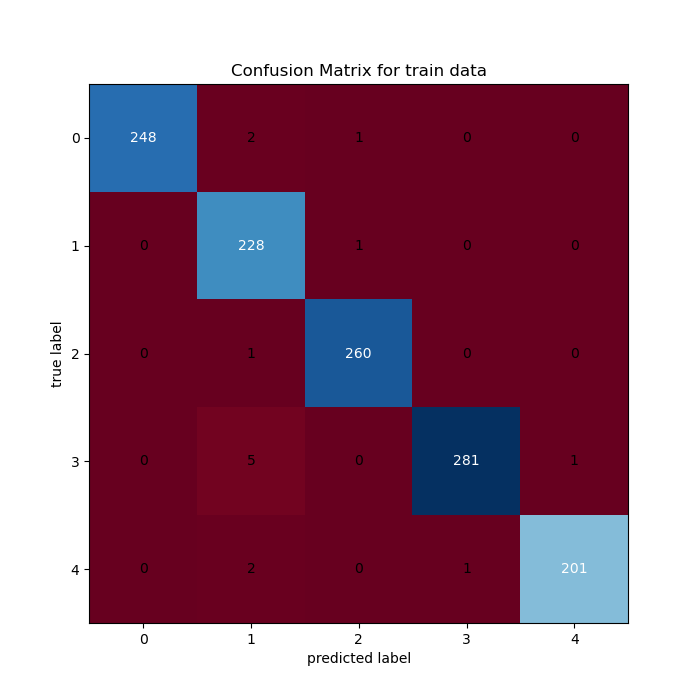
\includegraphics[height=2.5in]{Dataset_2a/dataset_2a_cmatrix_train_data_svc.png}
        \caption{Confusion Matrix for training data}
    \end{subfigure}%
    ~ 
    \begin{subfigure}[t]{0.5\textwidth}
        \centering
        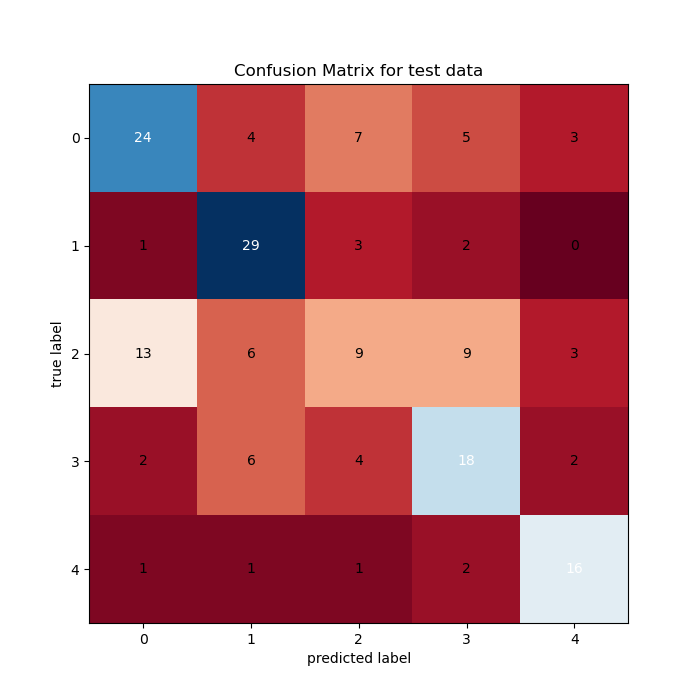
\includegraphics[height=2.5in]{Dataset_2a/dataset_2a_cmatrix_test_data_svc.png}
        \caption{Confusion Matrix for test data}
    \end{subfigure}%
    ~
    \caption{Confusion Matrix for the best model}
    \label{fig:13}
\end{figure}

%---------------------------------------------------------
\section{Varying Length Pattern Classification for Real World Data}


Dataset 2B consists of image histogram data pertaining to five class labels in which each image is represented by a set of 36, 23 dimensional vectors, i.e each image is represented by $36x23$ matrix. In the training phase each of row from the image matrices are treated as separate examples with the
same label as the parent image. In the classification phase, the classification of each image involves the calculating of the conditional probability that the image belongs to the class i as the product of the individual conditional probabilities of its constituent rows, i.e for an image matrix X and class label i.

 \begin{align*}
      p(y=y_i) &= \prod_{n=1}^{n} p(y=y_i) \\
                    &= \prod_{j=1}^{N}\sum_{k=1}^{K}w_{ik}. \mathcal{N}(x_n|\mu_{ik},c_{ik})
  \end{align*}
  

In both cases, the optimal model was found to be the cluster combination of [8,8,8,8,8] and a thorough search through the combination parameters were not feasible as the training of the model is computationally expensive across 150,000 data points

% -----------------------------------------------------------
{\rowcolors{3}{green!40!yellow!10}{green!0!yellow!30}
\begin{table}[!h]
\centering
\begin{tabular}{ |c|c|c|  }
\hline
\rowcolor{lightgray} Model & Training Accuracy & Val Accuracy \\
\hline
[1,1,1,1,1] & 23.13$\%$  & 22.88$\%$ \\   
 \hline
[2,2,2,2,2] & 45.77$\%$  & 47.17$\%$ \\ 
\hline
[3,3,3,3,3] & 57.62$\%$  & 47.45$\%$ \\
\hline
[4,4,4,4,4] & 61.85$\%$  & 51.97$\%$ \\
\hline
[5,5,5,5,5] & 67.37$\%$  & 61.58$\%$ \\
\hline
[6,6,6,6,6] & 69.64$\%$  & 62.42$\%$ \\
\hline
[7,7,7,7,7] & 70.21$\%$  & 66.10$\%$ \\
\hline
[8,8,8,8,8]  & 73.62 $\%$  & 66.66 $\%$ \\
\hline
\end{tabular}
\caption{Performance of models for Diagonal Covariance matrix}.
\label{table:9}
\end{table}
}

% -----------------------------------------------------------
{\rowcolors{3}{green!40!yellow!10}{green!0!yellow!30}
\begin{table}[!ht]
\centering
\begin{tabular}{ |c|c|c|  }
\hline
\rowcolor{lightgray} Model & Training Accuracy & Val Accuracy \\
\hline
[1,1,1,1,1] & 88.39$\%$  & 83.61$\%$ \\   
 \hline
[2,2,2,2,2] & 94.80$\%$  & 80.50$\%$ \\ 
\hline
[3,3,3,3,3] & 95.86$\%$  & 85.31$\%$ \\
\hline
[4,4,4,4,4] & 97.40$\%$  &  90.67 $\%$ \\
\hline
[5,5,5,5,5] & 98.86$\%$  & 94.63$\%$ \\
\hline
[6,6,6,6,6] & 99.02$\%$  & 94.63$\%$ \\
\hline
[7,7,7,7,7] & 99.26$\%$  & 94.35$\%$ \\
\hline
[8,8,8,8,8](optimal)  &  99.67 $\%$  & 95.19 $\%$ \\
\hline
\end{tabular}
\caption{Performance of models for Full Covariance matrix}.
\label{table:10}
\end{table}
}
\newpage




%------------------------------------------------------------
% \subsubsection*{Model Accuracy across combinations}

% \begin{figure}[!ht]
%     \centering
%     \begin{subfigure}[t]{0.5\textwidth}
%         \centering
%         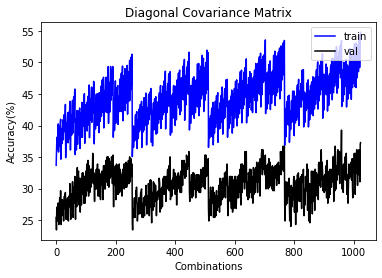
\includegraphics[height=2.5in]{Dataset_2a/diagonal covariance graph combinations.png}
%         \caption{Diagonal covariance combinations}
%     \end{subfigure}%
%     ~ 
%     \begin{subfigure}[t]{0.5\textwidth}
%         \centering
%         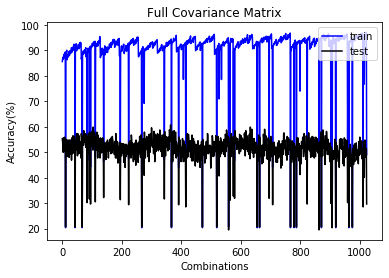
\includegraphics[height=2.5in]{Dataset_2a/full covariance graph combinations.png}
%         \caption{Full covariance combinations}
%     \end{subfigure}%
%     ~
%     \caption{Covariance Combinations}
%     \label{fig:23}
% \end{figure}


\begin{figure}[!h]
    \centering
    \begin{subfigure}[t]{0.5\textwidth}
        \centering
        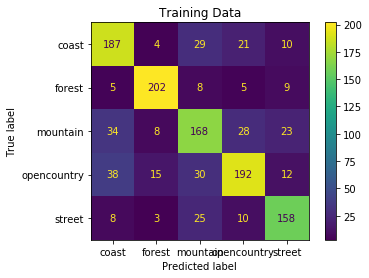
\includegraphics[height=2.5in]{Dataset_2b/diagonal covariance train confusion matrix.png}
        \caption{Train Data}
    \end{subfigure}%
    ~ 
    \begin{subfigure}[t]{0.5\textwidth}
        \centering
        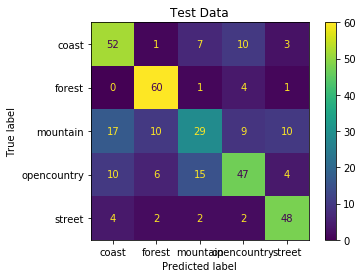
\includegraphics[height=2.5in]{Dataset_2b/diagonal covariance test confusion matrix.png}
        \caption{Validation Data}
    \end{subfigure}%
    ~
    \caption{Confusion Matrix for diagonal covariance}
    \label{fig:30}
\end{figure}

%------------------------------------------------------------
%\newpage

\begin{figure}[!h]
    \centering
    \begin{subfigure}[t]{0.5\textwidth}
        \centering
        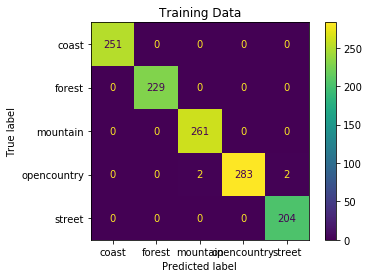
\includegraphics[height=2.5in]{Dataset_2b/full covariance train confusion matrix.png} 
        \caption{Train Data}
    \end{subfigure}%
    ~ 
    \begin{subfigure}[t]{0.5\textwidth}
        \centering
        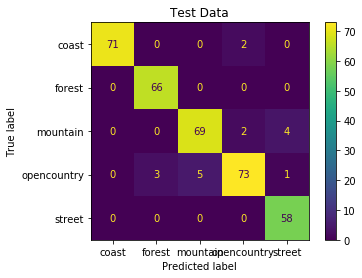
\includegraphics[height=2.5in]{Dataset_2b/full covariance test confusion matrix.png}
        \caption{Validation Data}
    \end{subfigure}%
    ~
    \caption{Confusion Matrix for full covariance}
    \label{fig:31}
\end{figure}





% ------------------------------------------------------------------------------
% End document
% ------------------------------------------------------------------------------
\end{document}